%======================================================================
\section{Resultados en el motor de Otto}
\label{sec:otto}
%======================================================================

\subsection{El frente cumple las dos hipótesis}

El frente de referencia del Otto se construyó uniendo un barrido denso de las cuatro variables con
todas las corridas de los algoritmos, y quedándose con los no dominados (unos 4\,800 puntos tras
adelgazar en una grilla de vóxeles). Sobre él:
\begin{itemize}
\item \textbf{(H1)}: mediana $\xi = 0.996$, máximo $1.005$. Satura la TUR.
\item \textbf{(H2)}: $\omega_h$, $r$ y los tiempos permiten mover $P$ y $\eta$ por separado; el
  frente llena una región del plano $(P,\eta)$ (Fig.~\ref{fig:lr}).
\end{itemize}
Y la predicción se cumple: el \textbf{91\%} del frente no es soportado en $(P,\eta,\Delta P)$, con
brechas de hasta $0.077$; en $(P,\Delta P,\Sigma)$ solo el \textbf{4\%}, con brechas menores que
$0.005$.

\subsection{El costo físico: ¿cuánto pierde un diseñador?}

La brecha $s^*$ es geométrica. Para traducirla a física (\code{scripts/costo\_fisico.py}), sea $S$ el
conjunto de motores alcanzables con una figura de mérito lineal (los soportados) y $p$ un motor del
frente. Definimos la \textbf{pérdida}
\begin{equation}
\varepsilon(p) = \min_{s\in S}\ \max\!\left(\frac{P_p}{P_s},\ \frac{\eta_p}{\eta_s},\
\frac{\Delta P_s}{\Delta P_p}\right) - 1 .
\end{equation}
Se lee así: el mejor motor que el diseñador puede obtener es, como mínimo, un $\varepsilon$ peor que
$p$ en algún objetivo (menos potencia, menos eficiencia o más fluctuaciones, en términos relativos).

\begin{center}
\begin{tabular}{lcc}
\toprule
Figura de mérito lineal en & $(P,\eta,\Delta P)$ & $(P,\Delta P,\Sigma)$\\
\midrule
fracción del frente alcanzable & 11\% & 98\% \\
pérdida $\varepsilon$ mediana & 14\% & 0\% \\
frente con $\varepsilon > 5\%$ & 75\% & 7\% \\
frente con $\varepsilon > 10\%$ & 60\% & 3\% \\
\bottomrule
\end{tabular}
\end{center}

\begin{figure}[h]
\centering
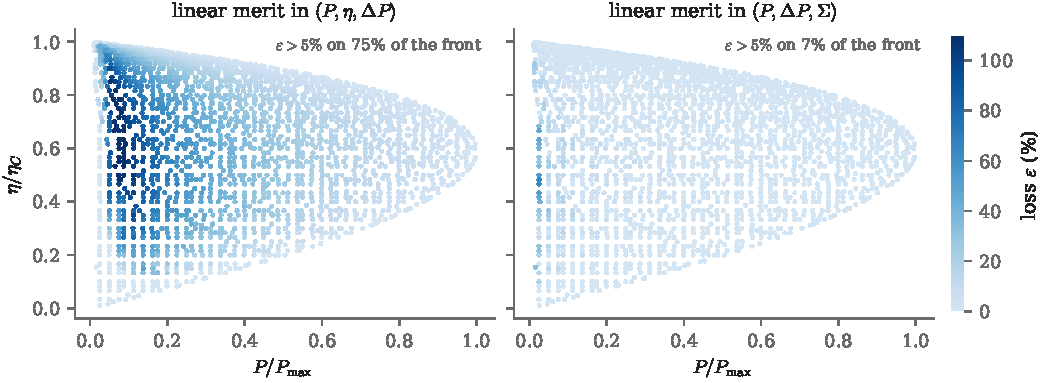
\includegraphics[width=\linewidth]{figs/fig2_cost.pdf}
\caption{Cada punto es un motor del frente en el plano $(P/\Pmax,\eta/\etaC)$, coloreado por la
pérdida $\varepsilon$. Izquierda: figura de mérito lineal en $\eta$. Derecha: en $\Sigma$.}
\label{fig:costo}
\end{figure}

\paragraph{Dónde se pierde.} Las pérdidas grandes se concentran a \textbf{baja potencia y eficiencia
media o alta} (mediana $P/\Pmax = 0.34$, $\eta/\etaC = 0.68$ entre los puntos con $\varepsilon > 5\%$):
los motores lentos, eficientes y de poco ruido. \textbf{Ejemplo extremo:} el motor con
$P/\Pmax = 0.075$ y $\eta/\etaC = 0.55$. Lo mejor que se puede obtener con una figura de mérito lineal
en $\eta$ tiene $\eta/\etaC = 0.24$ y $2.3$ veces sus fluctuaciones.

\paragraph{La recomendación física.} Escribir la figura de mérito con $\Sigma$ (como hacen Erdman
\emph{et al.}) recupera casi todo el frente de eficiencia.

\subsection{Los algoritmos y la descomposición de la pérdida}

Se compararon siete algoritmos evolutivos (sección~\ref{sec:algos}) con 30 semillas y $42\,000$
evaluaciones cada uno. La métrica principal es el \textbf{hipervolumen} (HV): el volumen del espacio
de objetivos dominado por las soluciones encontradas, hasta un punto de referencia. Más es mejor.

Para separar las dos razones por las que una suma ponderada puede perder HV, calculamos el HV de los
puntos soportados del frente de referencia. Es el \textbf{techo} de cualquier método de suma
ponderada, con los pesos que sea. Entonces:
\begin{itemize}
\item \textbf{pérdida por alcanzabilidad} $=$ HV(referencia) $-$ techo: lo que ningún peso recupera;
\item \textbf{pérdida por reparto} $=$ techo $-$ HV(MOEA/D-WS): lo que se pierde por cómo los pesos
  reparten las soluciones.
\end{itemize}

\begin{center}
\begin{tabular}{lcc}
\toprule
Otto, 30 semillas & $(P,\eta,\Delta P)$ & $(P,\Delta P,\Sigma)$\\
\midrule
HV del frente de referencia & 1.0810 & 1.2114\\
techo de cualquier suma ponderada & \textbf{0.9950} & 1.2113\\
\midrule
SMS-EMOA & 1.0425 & 1.1868\\
MOEA/D-AWA & 1.0404 & 1.1829\\
MOEA/D (Tchebycheff) & 1.0385 & 1.1744\\
NSGA-III & 1.0310 & 1.1700\\
RVEA & 1.0269 & 1.1683\\
NSGA-II & 1.0073 & 1.1612\\
MOEA/D-WS (suma ponderada) & 0.9670 & 1.1220\\
\midrule
pérdida WS: alcanzabilidad $+$ reparto & $\mathbf{0.086} + 0.028$ & $0.0001 + \mathbf{0.089}$\\
\bottomrule
\end{tabular}
\end{center}

\begin{idea}[Cómo leer la tabla]
La suma ponderada queda última en ambas formulaciones y pierde un HV parecido, pero \emph{por razones
distintas}. Con $\eta$, casi toda la pérdida es de alcanzabilidad: la silla. Seis de los siete
algoritmos, incluso NSGA-II, superan el techo de cualquier suma ponderada. Con $\Sigma$, la
alcanzabilidad es perfecta y toda la pérdida es de reparto: la degeneración por extensividad
(68 soluciones distintas de 105). La proposición predice exactamente esas dos cosas.
\end{idea}

\begin{figure}[h]
\centering
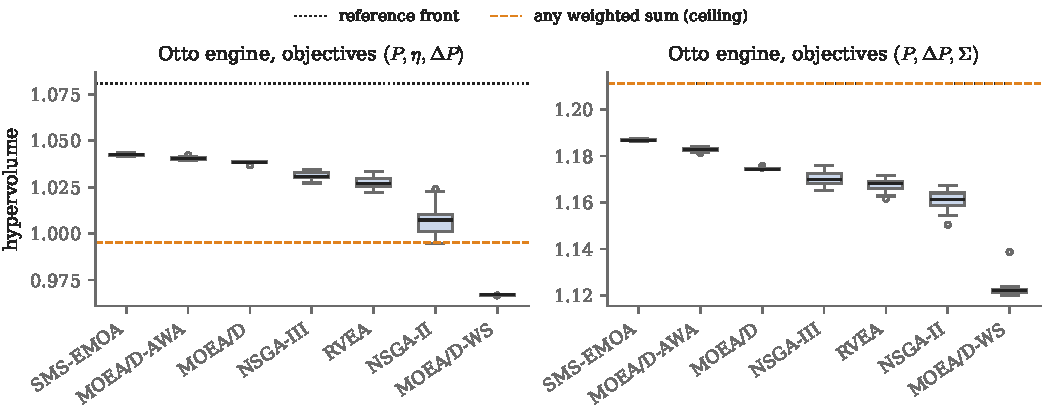
\includegraphics[width=\linewidth]{figs/fig3_hv_otto.pdf}
\caption{HV de los siete algoritmos en el Otto. Punteada: frente de referencia. Discontinua: techo
de cualquier suma ponderada. Con $\eta$ (izquierda) el techo queda por debajo de seis algoritmos;
con $\Sigma$ (derecha) coincide con la referencia.}
\end{figure}

%======================================================================
\section{Cuando la TUR se rompe: control por tramos}
\label{sec:tramos}
%======================================================================

\subsection{El modelo de Erdman}

Para ver qué pasa sin (H1) usamos el motor de punto cuántico de Erdman \emph{et al.} (2023):
$H(t) = u(t)E_0\sigma_z/2$, con relajación $\dot p = -\gamma\bigl[p - f(\beta(t)E_0u(t))\bigr]$,
$f(x) = 1/(1+e^x)$ (la misma forma de Gibbs/Fermi de la sección 2). Parámetros: $\beta_H = 1$,
$\beta_C = 2$, $E_0 = 2.5$, $u\in[0.2,1.1]$, $\gamma = 1$. El ciclo de duración $\tau$ se divide en
$N = 8$ tramos iguales; en cada uno se elige $u_k$ y \emph{con qué baño} se conecta. Son 17
variables (8 controles, 8 elecciones de baño y $\tau$). El Otto de cuatro tramos es un caso
particular, y el código lo reproduce con error $10^{-9}$ (\code{otto/piecewise.py}).

\subsection{Qué se observa}

\begin{itemize}
\item \textbf{La TUR se viola fuertemente}: el 81\% del frente tiene $\xi > 1$, con $\xi$ hasta
  $4$. El control libre permite ciclos que la cota estacionaria no cubre.
\item \textbf{La silla desaparece}: aunque el test marca como no soportado el 31\% ($\Sigma$) y el
  48\% ($\eta$) del frente, las brechas son diminutas (mediana $\approx 0.003$), y el techo de la
  suma ponderada queda a $0.1\%$ ($\Sigma$) y $0.2\%$ ($\eta$) del HV de referencia. El frente es
  casi convexo en ambas variables.
\item La suma ponderada sigue rindiendo distinto en $\eta$ que en $\Sigma$ (en $\Sigma$ queda segunda,
  detrás de SMS-EMOA), pero su pérdida ahora es \emph{toda de reparto}; la proposición no la explica.
\end{itemize}

\begin{center}
\begin{tabular}{lcc}
\toprule
Tramos, 30 semillas, 315\,000 evaluaciones & $(P,\eta,\Delta P)$ & $(P,\Delta P,\Sigma)$\\
\midrule
$\xi$ (mediana / máximo) & 1.59 / 4.04 & 1.45 / 4.02\\
HV referencia / techo & 1.1208 / 1.1184 & 1.2284 / 1.2276\\
SMS-EMOA / MOEA/D-AWA / MOEA/D-WS & 1.085 / 1.065 / 1.059 & 1.209 / 1.187 / 1.193\\
pérdida WS: alcanzabilidad $+$ reparto & $0.0024 + 0.060$ & $0.0008 + 0.035$\\
\bottomrule
\end{tabular}
\end{center}

\begin{idea}
El efecto geométrico está ligado a la saturación de la TUR: fuerte en el Otto (la alcanzabilidad se
lleva el 8\% del HV) y despreciable cuando el control libre rompe la cota. No es que ``la
suma ponderada con $\eta$ siempre falle'': falla cuando el frente es una superficie que satura la
TUR. Cómo interpola el efecto entre $\xi = 1$ y $\xi \gg 1$ es una pregunta abierta.
\end{idea}

%======================================================================
\section{Los algoritmos evolutivos}
\label{sec:algos}
%======================================================================

Esta parte es tu especialidad, así que va resumida y centrada en lo que importa para el argumento.

\subsection{Los siete algoritmos}

Todos usan población $N = 105$ (pesos de Das--Dennis con 13 divisiones para tres objetivos), cruce
SBX (probabilidad 1, $\eta_c = 20$) y mutación polinomial ($\eta_m = 20$).
\begin{itemize}
\item \textbf{NSGA-II}: ordenamiento no dominado más distancia de crowding; elitista.
\item \textbf{NSGA-III}: reemplaza el crowding por asociación a direcciones de referencia.
\item \textbf{SMS-EMOA}: estado estacionario; descarta el individuo con menor contribución al
  hipervolumen. Optimiza directamente la métrica con la que se evalúa, por eso suele ganar en HV.
\item \textbf{RVEA}: vectores de referencia con distancia penalizada por ángulo.
\item \textbf{MOEA/D}: descompone el problema en $N$ subproblemas escalares, uno por vector de pesos
  $w$, resueltos en paralelo con vecindarios (10\% de $N$, $\delta = 0.9$, $n_r = 2$). Usa
  \textbf{Tchebycheff normalizado}:
  \[ g^{\mathrm{te}}(x\mid w) = \max_i\ w_i\,\frac{f_i(x) - z_i^*}{z_i^{\mathrm{nad}} - z_i^*}. \]
\item \textbf{MOEA/D-AWA} (Qi \emph{et al.} 2014): MOEA/D más ajuste adaptativo de pesos. Transforma
  los pesos ($w_i \to (1/w_i)/\sum_j 1/w_j$) para que las direcciones de Tchebycheff queden uniformes,
  mantiene una población externa de no dominados (hasta $1.5N$) y, después del 80\% de la corrida,
  cada 10 generaciones elimina el 5\% de subproblemas en las zonas más pobladas y crea otros en las
  zonas más vacías (medidas con el producto de distancias a los vecinos más cercanos).
\item \textbf{MOEA/D-WS}: igual que MOEA/D pero con suma ponderada $g = \sum_i w_i\bar f_i$. Es la
  versión evolutiva de ``barrer los pesos de una figura de mérito lineal'': la línea base que el
  argumento necesita.
\end{itemize}

\subsection{Métricas y estadística}

\begin{itemize}
\item \textbf{HV}: volumen dominado, en coordenadas normalizadas por el frente de referencia, con
  punto de referencia $1.1$ en cada eje.
\item \textbf{IGD+}: distancia media desde los puntos del frente de referencia hasta la solución más
  cercana, contando solo las componentes en las que la solución es peor
  ($d^+(z,a) = \sqrt{\sum_i\max(a_i - z_i, 0)^2}$). Menos es mejor. MOEA/D-AWA tiene el mejor IGD+
  en el Otto en ambas formulaciones.
\item \textbf{Mann--Whitney U}: test no paramétrico (por rangos) para comparar las 30 corridas de cada
  algoritmo con MOEA/D-AWA.
\item \textbf{Holm}: corrección por comparaciones múltiples (seis tests). Se ordenan los $p$ y se
  multiplican por $(m - \text{rango})$, forzando monotonía. En el Otto todas las diferencias dan
  $p = 1.8\times10^{-10}$: separación completa de las 30 corridas (ninguna corrida de un algoritmo
  supera a ninguna del otro), que es el mínimo posible tras la corrección.
\end{itemize}

\subsection{Lo que pasó con DCE-MOEA/D}

Antes de esto se probó tu DCE-MOEA/D (en C++) en el Otto, con y sin el AWA de Qi. Su rendimiento
fue equivalente a MOEA/D-DE con el mismo AWA: la mejora venía del AWA, no del genotipo de gradiente.
Por eso el proyecto quedó con MOEA/D + AWA de Qi en Python.

%======================================================================
\section{Qué es nuevo, qué no, y qué diría un revisor}
%======================================================================

\paragraph{Ya se sabía.}
\begin{itemize}
\item Que la suma ponderada solo encuentra la envolvente convexa (desde los años 90).
\item Que los ciclos de Otto rápidos saturan la TUR (Erdman \emph{et al.} 2023).
\item Que los motores cíclicos pueden violar la TUR estacionaria (Holubec y Ryabov 2018).
\item Los frentes exactos en respuesta lineal (Almanza-Marrero \emph{et al.} 2026).
\end{itemize}

\paragraph{Lo que aporta el proyecto.}
\begin{itemize}
\item La conexión: saturación de la TUR $+$ frente bidimensional $\Rightarrow$ silla en $(P,\eta,\Delta P)$
  y tazón en $(P,\Delta P,\Sigma)$. Con demostración.
\item El costo físico medido en un modelo estándar (11\% alcanzable, 14\% de pérdida mediana).
\item La explicación de por qué la suma ponderada es exacta en respuesta lineal (el frente es una
  curva).
\item La descomposición alcanzabilidad/reparto, que separa la silla (con $\eta$) de la degeneración
  por extensividad (con $\Sigma$).
\end{itemize}

\paragraph{Críticas esperables.}
\begin{enumerate}
\item ``Es un corolario directo de un resultado clásico.'' Defensa: la generalización a
  $\Delta P = P\varphi(\eta)$ (sección~\ref{sec:legendre}) y el costo físico.
\item ``¿Quién comete el error?'' Erdman usa $\Sigma$ (bien); Almanza usa $\eta$ pero en respuesta
  lineal (donde es exacto). Hace falta encontrar trabajos que usen $\eta$ en una suma ponderada
  lejos del equilibrio.
\item ``El efecto depende de (H1), que es frágil'': con control libre desaparece.
\item ``El modelo no es cuántico'': no hay coherencias; el qubit es una cadena de Markov clásica. Lo
  cuántico es solo la discretización de niveles.
\end{enumerate}

%======================================================================
\section{Mapa del código y cómo reproducir}
%======================================================================

\begin{center}
\small
\begin{tabular}{p{0.36\linewidth}p{0.56\linewidth}}
\toprule
\textbf{Archivo} & \textbf{Qué hace (sección de esta guía)}\\
\midrule
\code{otto/model.py} & Gibbs, matrices $M$, ciclo límite, matriz inclinada, $P$, $\Delta P$, $\Sigma$, $\xi$, Monte Carlo (2--5)\\
\code{otto/problem.py} & Problemas de optimización: variables y objetivos $\eta$ o $\Sigma$ (6)\\
\code{otto/piecewise.py} & Modelo de Erdman por tramos (11)\\
\code{otto/moead.py} & MOEA/D, MOEA/D-AWA y MOEA/D-WS (12)\\
\code{otto/analysis.py} & Test de soporte por programación lineal, ec.~\eqref{eq:gap} (6)\\
\code{scripts/geometria.py} & Hessianos con sympy y superficie sintética (7)\\
\code{scripts/costo\_fisico.py} & Pérdida $\varepsilon$ y figura de costo (10)\\
\code{scripts/almanza.py} & Respuesta lineal (9)\\
\code{scripts/run\_piecewise.py} & Corre los 7 algoritmos (\code{--model otto} o tramos) (10--12)\\
\code{scripts/analyze\_piecewise.py} & HV, IGD+, tests, techo de suma ponderada (10--12)\\
\code{scripts/gap\_sensitivity.py} & Sensibilidad a la tolerancia del test (11)\\
\code{paper/make\_figures.py} & Figuras del paper\\
\code{docs/proposicion.md} & La proposición y la evidencia, en español\\
\bottomrule
\end{tabular}
\end{center}

\paragraph{Comandos} (desde \code{\textasciitilde/Projects/hidden-front}, con el entorno del proyecto):
{\small
\begin{verbatim}
.venv/bin/python -m pytest -q                       # 15 tests
.venv/bin/python scripts/geometria.py               # silla vs tazón
.venv/bin/python scripts/run_piecewise.py --model otto --seeds 30 --gens 400 --jobs 24
.venv/bin/python scripts/analyze_piecewise.py --model otto
.venv/bin/python scripts/costo_fisico.py
.venv/bin/python scripts/almanza.py
.venv/bin/python scripts/run_piecewise.py --seeds 30 --gens 3000 --jobs 24
.venv/bin/python scripts/refine_reference.py
.venv/bin/python scripts/analyze_piecewise.py
\end{verbatim}
}

%======================================================================
\section{Ejercicios}
%======================================================================

\newcounter{ejer}
\newcommand{\ejercicio}[2]{\par\medskip\refstepcounter{ejer}\label{#1}\noindent\textbf{Ejercicio \theejer\ (#2).}\ }

\ejercicio{ej:gibbs}{Gibbs} Deduce $a = 1/(1+e^{\omega/T})$ a partir de la función de partición de un
sistema de dos niveles.

\ejercicio{ej:ciclolimite}{ciclo límite} A partir de $p_1 = a_h + (p_2 - a_h)x_h$ y
$p_2 = a_c + (p_1 - a_c)x_c$, deduce $p_1$ y la ec.~\eqref{eq:dp} para $p_1 - p_2$.

\ejercicio{ej:numerico}{números} Con $\omega_h = 2.035$, $\omega_c = 1.433$, $\tau_h = \tau_c = 0.675$,
$\tau_q = 0.05$, $T_h = 1$, $T_c = 0.5$, $\gamma = 1$, calcula $p_1 - p_2$, $W$, $P$, $\eta$ y $\Sigma$.
Con $\Delta P = 0.0126$, calcula $\xi$.

\ejercicio{ej:sigma}{producción de entropía} Demuestra que $\Sigma = P(\etaC - \eta)/(\eta T_c)$.

\ejercicio{ej:tur}{TUR de motores} Partiendo de $\Delta P\,\Sigma \ge 2P^2$, deduce
$\eta \le \etaC/(1 + 2T_cP/\Delta P)$.

\ejercicio{ej:correl}{correlaciones} ¿Por qué $\theta''(0)$ no es igual a la varianza del trabajo de
un solo ciclo? ¿Con qué rapidez decaen las correlaciones entre ciclos?

\ejercicio{ej:hess}{hessianos} Calcula el hessiano de $h(P,\Sigma) = 2P^2/\Sigma$ y muestra que es
semidefinido positivo con dirección nula $(P,\Sigma)$. Verifica que $h$ es homogénea de grado 1.

\ejercicio{ej:escala}{invariancia de escala} Muestra que si $f_i\to\alpha_if_i + \beta_i$ con
$\alpha_i > 0$, los puntos soportados no cambian.

\ejercicio{ej:tcheby}{Tchebycheff} Sea $p$ un punto de Pareto y $z$ un punto ideal con $z_i < f_i(p)$.
Muestra que con $w_i \propto 1/(f_i(p) - z_i)$, $p$ minimiza $\max_i w_i(f_i - z_i)$.

\ejercicio{ej:lr}{respuesta lineal} Con $P = -y(y+q)$, $\bar\eta = -y(y+q)/(1+qy)$ y
$\Sigma = 1+2qy+y^2$, $y\in(-q,0)$, muestra que aumentar $q$ mejora los tres objetivos. Muestra que
con $q = 1$ el frente satura la TUR.

\ejercicio{ej:silla}{intuición} Toma $z = xy$. Muestra que ningún plano $z = \alpha x + \beta y + c$
puede quedar por debajo de la superficie en un entorno de un punto, y que sin embargo la curva
$\{(t,t,t^2)\}$ contenida en ella es convexa. Relaciónalo con (H2).

%======================================================================
\section{Soluciones}
%======================================================================

\textbf{\ref{ej:gibbs}.} $Z = 1 + e^{-\omega/T}$, así que
$p_{\mathrm{eq}} = e^{-\omega/T}/Z = 1/(e^{\omega/T} + 1)$.

\textbf{\ref{ej:ciclolimite}.} Sustituyendo la segunda en la primera:
$p_1 = a_h(1-x_h) + x_h a_c(1-x_c) + x_hx_c\,p_1$, luego
$p_1 = [a_h(1-x_h) + x_ha_c(1-x_c)]/(1 - x_hx_c)$. Además $p_1 - p_2 = (1-x_c)(p_1 - a_c)$ y
$p_1 - a_c = (a_h - a_c)(1-x_h)/(1-x_hx_c)$ (los términos con $a_c$ se agrupan como
$a_c[x_h - x_hx_c - 1 + x_hx_c] = -a_c(1-x_h)$).

\textbf{\ref{ej:numerico}.} $a_h = 0.1156$, $a_c = 0.0539$, $x_h \approx x_c \approx 0.509$.
$p_1 - p_2 = 0.0617\times0.2408/0.7406 = 0.0201$. $W = 0.602\times0.0201 = 0.0121$,
$\tau_{\mathrm{ciclo}} = 1.45$, $P = 0.00833$, $\eta = 1 - 1.433/2.035 = 0.296$,
$\Sigma = 0.0201\,(2.866 - 2.035)/1.45 = 0.0115$.
$\xi = 2P^2/(\Delta P\,\Sigma) = 1.39\times10^{-4}/1.45\times10^{-4} = 0.96$.

\textbf{\ref{ej:sigma}.} En tasas, $\dot Q_h = P/\eta$ y $\dot Q_c = \dot Q_h - P = P(1-\eta)/\eta$.
Entonces $\Sigma = \dot Q_c/T_c - \dot Q_h/T_h = \frac{P}{\eta}\bigl[\frac{1-\eta}{T_c} - \frac{1}{T_h}\bigr]
= \frac{P}{\eta T_c}\bigl[1 - \eta - \frac{T_c}{T_h}\bigr] = \frac{P(\etaC-\eta)}{\eta T_c}$.

\textbf{\ref{ej:tur}.} $\Delta P\,P(\etaC-\eta)/(\eta T_c) \ge 2P^2 \Rightarrow \Delta P(\etaC-\eta)\ge
2T_cP\eta \Rightarrow \eta(\Delta P + 2T_cP) \le \Delta P\,\etaC$, y se divide por $\Delta P$.

\textbf{\ref{ej:correl}.} $v = \operatorname{Var}(w) + 2\sum_{j\ge1}\operatorname{Cov}(w_0,w_j)$: el
estado al final de un ciclo condiciona el siguiente. Las covarianzas decaen con el segundo autovalor
de la matriz de un ciclo, que es $D = x_hx_c$: $\operatorname{Cov}(w_0,w_j)\propto (x_hx_c)^{j}$.
Contactos largos ($x\to0$) borran la memoria; contactos cortos la alargan.

\textbf{\ref{ej:hess}.} $h_{PP} = 4/\Sigma$, $h_{P\Sigma} = -4P/\Sigma^2$, $h_{\Sigma\Sigma} = 4P^2/\Sigma^3$.
Traza positiva y determinante $16P^2/\Sigma^4 - 16P^2/\Sigma^4 = 0$: semidefinido positivo.
$\nabla^2h\,(P,\Sigma)^\top = (4P/\Sigma - 4P/\Sigma,\ -4P^2/\Sigma^2 + 4P^2/\Sigma^2) = 0$.
$h(\lambda P,\lambda\Sigma) = 2\lambda^2P^2/(\lambda\Sigma) = \lambda h$.

\textbf{\ref{ej:escala}.} $\sum_iw_i(\alpha_if_i + \beta_i) = \sum_i(w_i\alpha_i)f_i + \text{cte}$.
Con $w'_i = w_i\alpha_i/\sum_jw_j\alpha_j \ge 0$, el minimizador es el mismo.

\textbf{\ref{ej:tcheby}.} Con esos pesos, $w_i(f_i(p) - z_i) = c$ igual para todo $i$, así que el
valor en $p$ es $c$. Si existiera $q$ con $\max_iw_i(f_i(q) - z_i) < c$, tendríamos
$f_i(q) < f_i(p)$ para todo $i$: $q$ dominaría a $p$, contradicción.

\textbf{\ref{ej:lr}.} $\partial_qP = -y > 0$; $\partial_q\Sigma = 2y < 0$;
$\partial_q\bar\eta = -y(1-y^2)/(1+qy)^2 > 0$ para $y\in(-1,0)$. Con $q = 1$, $e = -y$:
$\sigma_P^2\Sigma = 2e^2(1-e)^2 = 2P^2$.

\textbf{\ref{ej:silla}.} El hessiano de $xy$ es $\bigl(\begin{smallmatrix}0&1\\1&0\end{smallmatrix}\bigr)$,
con autovalores $\pm1$; a lo largo de $x = -y$ la superficie cae por debajo de cualquier plano
tangente. Pero sobre la curva $x = y = t$ vale $z = t^2$, convexa. Una curva sobre una silla puede ser
convexa; por eso (H2) es necesaria. Es lo que pasa en respuesta lineal.

%======================================================================
\section{Glosario}
%======================================================================

\begin{description}[style=nextline,leftmargin=1.2em]
\item[Brecha $\omega$] Diferencia de energía entre los dos niveles del qubit; hace el papel del volumen.
\item[Ciclo límite] Régimen periódico al que llega el qubit tras pocos ciclos.
\item[Estadística de conteo completa] Cálculo de todos los cumulantes de una cantidad acumulada
  (trabajo) con una matriz inclinada.
\item[Función generadora escalada $\theta(\chi)$] $\lim\frac1n\ln\langle e^{\chi W_n}\rangle$; el
  ``$\ln Z$'' del trabajo.
\item[Producción de entropía $\Sigma$] Entropía generada en los baños por unidad de tiempo; cero si y
  solo si el motor es reversible ($\eta = \etaC$).
\item[TUR] $\Delta P\,\Sigma\ge2P^2$: el ruido relativo está acotado por la disipación.
\item[$\xi$] $2P^2/(\Delta P\,\Sigma)$; $\xi = 1$ es saturar la TUR.
\item[Frente de Pareto] Conjunto de compromisos no dominados entre los objetivos.
\item[Punto soportado] Punto del frente que minimiza alguna suma ponderada con pesos no negativos.
\item[Techo de suma ponderada] HV de los puntos soportados: lo máximo que puede lograr un método de
  suma ponderada.
\item[Silla / tazón] Superficie con hessiano indefinido / semidefinido positivo.
\item[Inequivalencia de ensambles] Cuando el ensamble canónico no reproduce estados del
  microcanónico porque $S(E)$ no es cóncava.
\item[Respuesta lineal] Régimen cercano al equilibrio con flujos lineales en las fuerzas (Onsager).
\end{description}

%======================================================================
\section*{Referencias principales}
\addcontentsline{toc}{section}{Referencias principales}
%======================================================================
\begin{itemize}\small
\item A.~C. Barato y U. Seifert, Phys. Rev. Lett. \textbf{114}, 158101 (2015). (TUR)
\item T.~R. Gingrich, J.~M. Horowitz, N. Perunov y J.~L. England, Phys. Rev. Lett. \textbf{116}, 120601 (2016).
\item P. Pietzonka y U. Seifert, Phys. Rev. Lett. \textbf{120}, 190602 (2018). (TUR de motores)
\item V. Holubec y A. Ryabov, Phys. Rev. Lett. \textbf{121}, 120601 (2018). (motores cíclicos)
\item P.~A. Erdman \emph{et al.}, Phys. Rev. Research \textbf{5}, L022017 (2023). (frentes con RL, modelo por tramos)
\item J.~A. Almanza-Marrero, É. Roldán y G. Manzano, arXiv:2603.19885 (2026). (respuesta lineal)
\item F.~L. Curzon y B. Ahlborn, Am. J. Phys. \textbf{43}, 22 (1975).
\item H. Touchette, Phys. Rep. \textbf{478}, 1 (2009). (grandes desviaciones)
\item I. Das y J.~E. Dennis, Struct. Optim. \textbf{14}, 63 (1997). (límites de la suma ponderada)
\item M. Ehrgott, \emph{Multicriteria Optimization}, Springer (2005).
\item S. Boyd y L. Vandenberghe, \emph{Convex Optimization}, Cambridge (2004). (funciones perspectiva)
\item Q. Zhang y H. Li, IEEE Trans. Evol. Comput. \textbf{11}, 712 (2007). (MOEA/D)
\item Y. Qi \emph{et al.}, Evol. Comput. \textbf{22}, 231 (2014). (MOEA/D-AWA)
\end{itemize}
